\tikzset{>=latex} % for LaTeX arrow head
\contourlength{1.2pt}

\pgfmathdeclarefunction{gauss}{3}{%
  \pgfmathparse{1/(#3*sqrt(2*pi))*exp(-((#1-#2)^2)/(2*#3^2))}%
}
\pgfmathdeclarefunction{cdf}{3}{%
  \pgfmathparse{1/(1+exp(-0.07056*((#1-#2)/#3)^3 - 1.5976*(#1-#2)/#3))}%
}
\pgfmathdeclarefunction{fq}{3}{%
  \pgfmathparse{1/(sqrt(2*pi*#1))*exp(-(sqrt(#1)-#2/#3)^2/2)}%
}
\pgfmathdeclarefunction{fq0}{1}{%
  \pgfmathparse{1/(sqrt(2*pi*#1))*exp(-#1/2))}%
}

\colorlet{mydarkblue}{blue!30!black}

\usepgfplotslibrary{fillbetween}
\pgfplotsset{compat=1.12} % TikZ coordinates <-> axes coordinates


\def\N{50}

% GAUSSIANs: basic properties





% GAUSSIANs: p-value, PLR


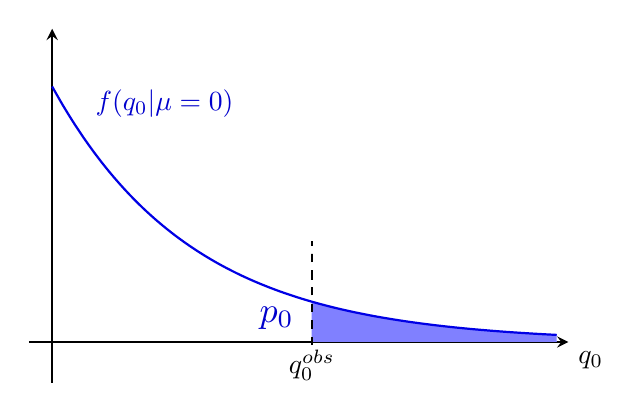
\begin{tikzpicture}
  \message{p-value, PLR^^J}
  
  \def\q{4.8}
  \def\Bs{2.6}
  \def\xmax{1.8*\q}
  \def\ymin{{-0.16/\Bs}}
  \def\ymax{{1.1/\Bs}}
  
  \begin{axis}[every axis plot post/.append style={
               mark=none,domain=0:{1.08*\xmax},samples=\N,smooth},
               xmin={-0.05*(\xmax)}, xmax=\xmax,
               ymin=\ymin, ymax=\ymax,
               axis lines=middle,
               axis line style=thick,
               enlargelimits=upper, % extend the axes a bit to the right and top
               ticks=none,
               xlabel=$q_0$,
               every axis x label/.style={at={(current axis.right of origin)},anchor=north west},
               y=240pt,
               domain=0:(\xmax)
              ]
    
    % PLOTS
    \addplot[name path=B,thick,black!10!blue] {exp(-x/\Bs)/\Bs};
    \addplot[black,dashed,thick]
      coordinates {(\q,{-0.08*exp(-\q/\Bs)/\Bs}) (\q, {2.5*exp(-\q/\Bs)/\Bs})}
      node[below=-2pt,pos=0] {$q_0^\text{obs}$};
    
    % FILL
    \path[name path=xaxis]
      (0,0) -- (1.08*\xmax,0);
    \addplot[white!50!blue] fill between[of=xaxis and B, soft clip={domain=\q:1.08*\xmax}];
    
    % LABELS
    \node[above right=2pt,black!20!blue] at ( 0.2*\Bs,{exp(-0.2)/\Bs}) {$f(q_0|\mu=0)$};
    \node[left,black!20!blue,scale=1.3] at ({0.98*\q},{0.6*exp(-\q/\Bs)/\Bs}) {$p_0$};
    
  \end{axis}
\end{tikzpicture}
